\chapter{可重构模块硬件实现}

本章详细阐述构成动态可重构矩阵乘法加速系统核心计算能力的可重构模块(RM)的设计与实现过程。
这些模块是专门为加载到第三章定义的三个可重构分区(RP)中而设计的。我们将采用Xilinx Vitis 高层次综合(HLS)工具,利用C/C++语言进行算法描述和硬件优化。
对于每个关键的RM(稀疏矩阵解压、稠密矩阵乘法、稀疏矩阵压缩),
本章将覆盖其核心算法分析、HLS实现策略、接口设计、关键优化技术以及最终的综合与实现结果
(基于目标平台Xilinx Kria KV260的Zynq UltraScale+ MPSoC PL部分的资源特性)。

\section{Vitis HLS 设计方法论概述}

Vitis HLS作为一种高层次综合工具,允许设计者使用C、C++或OpenCL C等高级语言描述硬件行为,
然后将其自动转换为寄存器传输级(RTL)代码。这种方法显著提高了设计效率,使得复杂的算法能够更快地在FPGA上实现。
在本系统中,所有可重构模块均采用C/C++进行开发。核心设计策略是首先实现算法的功能正确性,然后通过迭代地应用HLS优化指令(pragmas)来提升性能和资源利用率。
关键的优化指令包括用于实现指令级并行的 \verb|PIPELINE| 指令,用于循环展开以实现数据级并行的 \verb|UNROLL| 指令,
用于优化存储器访问的 \verb|ARRAY_PARTITION| 指令,以及用于定义模块接口的 \verb|INTERFACE| 指令。
设计目标是为每个RM生成高效的、能够充分利用FPGA并行性和流水线性质的硬件实现。

\section{稀疏矩阵解压/压缩模块}

稀疏矩阵解压模块负责将以特定稀疏格式存储的矩阵转换为稠密矩阵格式。
其核心算法依赖于稀疏格式的定义。以CSR(Compressed Sparse Row)格式为例,
输入数据通常包括值数组(values)、列索引数组(column indices)和行指针数组(row pointers)。
稀疏矩阵压缩模块的功能与解压模块相反,它将稠密矩阵转换为指定的稀疏格式。

稀疏矩阵解压模块的算法逻辑是遍历行指针数组,确定每行非零元素的数量和位置,
然后根据列索引数组和值数组将这些非零元素填充到稠密矩阵的相应位置,
其余位置则填充零。在HLS实现中,通常会涉及嵌套循环:外层循环遍历行,
内层循环遍历该行内的非零元素。为了高效访问输入稀疏数据(通常存储在主存中),
模块通过AXIMM主接口读取。输出的稠密矩阵同样通过AXIMM主接口写回主存,或者通过AXIS接口流式传输给下一个处理模块。
输入输出的接口选择由数据选择器实现,其选择信号由主机程序指定,并在传输矩阵数据前先行传至FPGA上。

稀疏矩阵压缩模块模块首先遍历输入的稠密矩阵,识别所有非零元素,并记录它们的值和索引。
随后,根据目标稀疏格式(如CSR)的要求,将这些信息组织成相应的数组结构。
例如,生成CSR格式需要统计每行的非零元素个数以构建行指针数组,同时记录非零元素的值和列索引。

\section{稠密矩阵乘法模块}

\begin{figure}[htbp]
\centerline{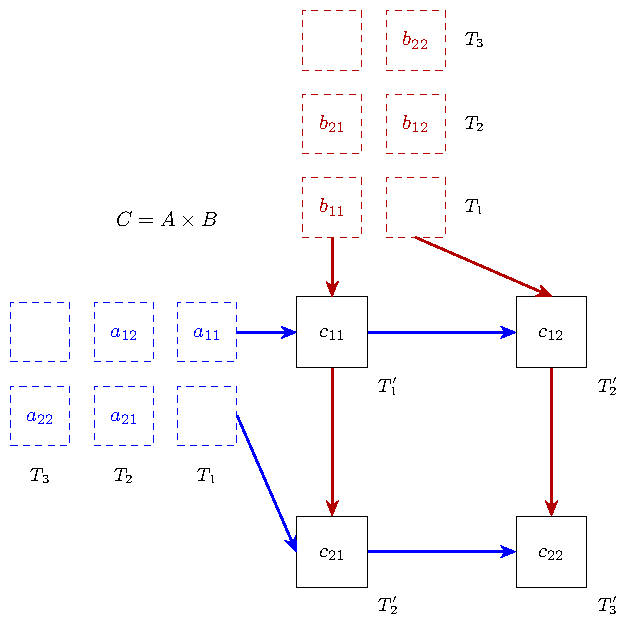
\includegraphics[width=0.8\columnwidth]{figures/systolic}}
\caption{脉动阵列算法作用于2\texttimes{}2矩阵乘法。}
\label{fig:systolic}
\end{figure}

稠密矩阵乘法模块是本加速系统的核心计算单元之一,其设计采用了脉动阵列(Systolic Array)结构,并结合分块(Tiling)策略以处理大规模矩阵。

如图\ref{fig:systolic}所示,在矩阵乘法\(C=A\times B\)的脉动阵列算法中,每个PE计算矩阵\(C\)的对应元素,其从左侧和上方接收矩阵\(A\)和矩阵\(B\)的元素,
并在下一时钟周期传递给右侧和下方的PE。PE将每个时钟周期输入的元素相乘并累加,最终便得到了矩阵\(C\)的元素值。
输入矩阵\(A\)和\(B\)分别对行和列进行 \verb|ARRAY_PARTITION|(如此便能对不同行/列的元素并行访问),每行/列相较于上一行/列延迟一个周期送入PE。

脉动阵列因其规整的数据流和高度的并行性,非常适合在FPGA上实现矩阵乘法。
算法将输入矩阵A和B分割成小块(tiles),然后将这些小块数据送入脉动阵列进行计算。
每个处理单元(Processing Element, PE)在脉动阵列中执行乘加运算。分块策略有助于管理片上存储资源(如BRAM),
使得模块可以处理远大于片上存储容量的矩阵。HLS实现中,需要精心设计数据加载、PE阵列的计算逻辑以及结果写回的控制流程。

针对脉动阵列的PEs,其内部的乘加操作循环体应用 \verb|PIPELINE| 指令是标准做法,由Vitis自动处理而无需手动设置。
为了实现PE之间的数据并行流动,相关的循环通常会被完全 \verb|UNROLL|。
用于缓存输入矩阵分块的片上存储器(BRAMs)会使用 \verb|ARRAY_PARTITION| 指令进行分区,
以提供足够的并行读写带宽。
接口方面,输入矩阵数据(或其分块)通常通过AXIS从接口输入,这便于从前级模块(如解压模块)或PS端高效接收数据。
计算结果(稠密矩阵或其分块)通过AXIS主接口输出,可以流向后级模块(如压缩模块)或PS端。
对于直接从主存加载分块或写回分块的场景,也会配置AXIMM主接口。输入输出的接口选择同样由数据选择器实现。

\section{模块间的协同与动态特性}

以上设计的可重构模块均具备标准的AXI接口(AXIMM用于内存访问,AXIS用于流式数据传输),
这使得它们不仅可以独立工作,也可以在FPGA的三个可重构分区中灵活组合,
通过AXIS接口形成高效的数据处理流水线。例如,稀疏矩阵乘法任务可以通过动态加载稀疏解压RM、稠密乘法RM和稀疏压缩RM,
并使它们通过AXIS接口依次串联工作。
每个RM都作为独立的编译单元生成部分比特流,为第三章所述的动态重构系统提供了基础。
